\documentclass[a4paper,10pt]{article}

% Lenguaje
\usepackage[spanish]{babel}
\usepackage[utf8]{inputenc}
\setlength{\parindent}{0pt}

% Ajustes documento
\usepackage{geometry}
\geometry{left=3cm,right=3cm,top=3cm,bottom=3cm,headheight=1cm,headsep=0.5cm}
\usepackage{enumitem}

\usepackage{xcolor}
\usepackage{hyperref}
\hypersetup{
    colorlinks=true,
    linkcolor=[rgb]{0.149 0 0.3216},
    filecolor=magenta,      
    urlcolor=blue,
    citecolor=blue,
}
\urlstyle{same}

\usepackage{amsmath}

% Incluir gráficos
\usepackage{graphicx}
\usepackage{float}

% Sangrado y espacio entre párrafos
\setlength{\parskip}{1em}
\setlength{\parindent}{1.5em}

% Portada
\title{Diseño y construcción de un sistema para adquisición y análisis
  del consumo energético en el hogar}
\author{Jesús Sánchez de Lechina Tejada}
\date{Junio 2020}

\begin{document}
\maketitle
\thispagestyle{empty}
\begin{center}
  \includegraphics[scale=0.4]{img/logo_ugr.pdf}
\end{center}

\newpage

\tableofcontents

\newpage

\section{Internet de las Cosas}\label{internet-de-las-cosas}

Uno de los términos más recurrentes en el ámbito de la tecnología a día
de hoy es el de \textit{``Internet de las Cosas''} (en inglés, IoT, \textit{Internet of
Things}). Pero, puesto que el término puede resultar ambiguo, es
conveniente dar una definición sobre esta que permita esclarecer el
concepto.

El Internet de las Cosas es un paradigma tecnológico en sí mismo.
Desglosándo el concepto vemos que reúne dos tecnologías. Por un lado
parte de ``las cosas'', que abarca desde los dispositivos y
electrodomésticos que podemos encontrar en nuestro día a día; que tienen
una funcionalidad en sí misma (p.ej. una televisión, un frigorífico),
hasta incluso podemos abstraer a personas o animales (una persona con un
marcapasos, un ave con un geolocalizador u otros
ejemplos\cite{iotagendawebsiteWhatInternetThings}). A estas ``cosas''
se les añade el término
``Internet'', que no es más que una abstracción de la conectividad que
permite dotar a las cosas de comunicación con el exterior, extendiendo
sus funcionalidades sin privarlas de su cometido original. Esta es
su principal característica, la posibilidad de comunicación con otras
``cosas'' mediante internet y sin la necesidad de intervención humana.

La idea que trasciende de esto es que cualquier cosa o dispositivo que
usemos habitualmente puede conectarse a una red, a internet. Haciendo
que, en términos de redes, un dispositivo IoT se pueda equiparar a un
ordenador convencional.

\subsection{¿Qué es un dispositivo
IoT?}\label{quuxe9-es-un-dispositivo-iot}

En el símil anterior hemos adelantado el concepto de dispositivo IoT sin
llegar a definirlo completamente. A continuación explicaremos qué es
concretamente un dispositivo IoT y qué lo diferencia de otras ``cosas''.

Un dispositivo IoT es una entidad (objeto, o incluso animales o
personas) que tiene una funcionalidad en sí misma y a la cual dotamos de
una capacidad de conexión y telecomunicación. De modo que sea capaz de,
por sí misma, comunicarse con otros dispositivos en su entorno dotados
de esta misma capacidad.

Los beneficios que podemos obtener de este paradigma se pueden aplicar
en muchas áreas\cite{vongsingthongs.;smanchats.IoTExamplesSuranaree},
por ejemplo:

\begin{itemize}
\item
  Logística: Rastreo de envíos por correo o estado del stock en
  almacenes automatizando lectura de los items mediante wifi.
\item
  Transporte: Gestión automática de rutas por GPS; captura y procesado
  de infracciones de velocidad.
\item
  Salud: Desde una pulsera que capte tus hábitos de vida hasta
  la supervisión de personas ancianas que viven solas.
\item
  Monitorización: Desde instalación de sensores en un bosque para medir
  datos de contaminación hasta medir en un hogar el consumo de un
  electrodoméstico.
\end{itemize}

Este último ejemplo es justo la motivación de nuestro trabajo. Podemos
usar esta tecnología para crear un \textbf{enchufe inteligente} que
nos permita saber nuestro consumo eléctrico y controlar el uso que le
damos.

\newpage

\section{Revisión de enchufes inteligentes existentes en el
mercado}\label{revisiuxf3n-de-enchufes-inteligentes-existentes-en-el-mercado}

\subsection{¿Qué es un enchufe? Tipos de
enchufe}\label{quuxe9-es-un-enchufe-tipos-de-enchufe}

Un enchufe es una fuente de alimentación entre sistemas eléctricos. En
este proyecto trataremos los enchufes dentro del ámbito doméstico o
comercial frente al ámbito industrial, que tiende a trabajar con
voltajes de un orden muy superior.

Un enchufe en el ámbito doméstico permite la conexión entre un
dispositivo electrónico y la corriente alterna para la alimentación de
este dispositivo.

Estos trabajan con unos voltajes entre 100V y
240V.\cite{iecIECWorldPlugs} El tipo de enchufe, voltaje y frecuencia
usados en una región geográfica vienen determinados por un convenio
fijado por el gobierno de esa zona.

Por razones históricas\cite{nuevatribunaOrigenFrecuenciasElectricas}
no existe una estandarización.

Trabajaremos con el tipo de enchufe usado en España, que cuenta con un
potencial de 230V y una frecuencia de 50Hz\cite{IECWorldPlugs}.


\subsection{¿Qué es un enchufe
inteligente?}\label{quuxe9-es-un-enchufe-inteligente}

Un enchufe inteligente extiende esta definición de enchufe. Actuando
como una interfaz que permite añadir un amplio abanico de
funcionalidades relativas al manejo y supervisión de estos dispositivos
externos. Dotándole de las ventajas de la conectividad.

Esto encaja con la definición de dispositivo IoT que mencionábamos
previamente. Un objeto cotidiano que ha sido dotado de la capacidad de
comunicación con otros dispositivos.

\subsection{Funcionalidades comunes que ofertan los enchufes
electrónicos
actualmente}\label{funcionalidades-comunes-que-ofertan-los-enchufes-electruxf3nicos-actualmente}

\subsubsection{Monitorización:}\label{monitorizaciuxf3n}

Supervisar el uso de energía: Esto permite establecer un control sobre
su uso, realizar estimaciones sobre el coste o incluso notificar frente
a anomalías como el consumo en horarios no esperados o picos de voltaje.

\subsubsection{Control:}\label{control}

Manejar tus dispositivos de manera remota, programar el horario de
funcionamiento de estos o la manera en la que funcionan son solo algunas
de las opciones; destacando la posibilidad de integración con otros
dispositivos que proporcionen una mayor accesibilidad (p.ej. la interfaz
de voz de un asistente de móvil).

\subsection{Tipos de enchufes}\label{tipos-de-enchufes}

Atendiendo a sus características más distintivas podemos hacer una
clasificación (no excluyente) de:

\begin{itemize}
\item
  Enchufes inteligentes (E.I.) por control remoto (wifi, bluetooth,
  infrarrojos u otros tipos de señales electromagnéticas).
\item
  E.I. programables, aquellos que permiten la progamación temporal de eventos.
\item
  E.I. de regletas, aquellos que permiten tratar con varios
  dispositivos simultáneamente en un mismo enchufe.
\end{itemize}

\subsection{Modelos en el mercado}\label{modelos-en-el-mercado}

La comercialización de este producto está muy extendida, proporcionando
una amplia oferta de productos los cuales podemos recoger bajo la
clasificación previa:

\begin{itemize}
\item
  Programación temporal: Permiten la ejecución de tareas a horas
  concretas del día. Por ejemplo:
  \href{https://web.archive.org/web/20191111121153/https://www.amazon.es/Garza-Power-Temporizador-anal\%C3\%B3gico-programaci\%C3\%B3n/dp/B00URUVDW2/}{Garza
  400603 (analógico)},
  \href{https://web.archive.org/web/20191112121450/https://www.amazon.es/dp/B00ZJ1LQDK}{Orbegozo
  PG 20 (digital)}
\item
  Control remoto: Se pueden controlar con mando a distancia, a través de
  una app o con control por voz. Por ejemplo:
  \href{https://web.archive.org/web/20191112130933/https://www.amazon.es/dp/B06W586CDZ}{TP-Link
  HS100} o la
  \href{https://web.archive.org/web/20191116174434/https://www.amazon.es/dp/B07DJ2G1CW}{Regleta
  Xiaomi}, que es un ejemplo de intersección entre E.I. de regleta y por
  control remoto.
\end{itemize}

\newpage

\section{Arquitecturas IoT}\label{arquitecturas-iot}

El paradigma de IoT viene a integrarse entre los mecanismos
convencionales y el resto de redes. En sus primeros pasos se adaptaron
sus diseños a las necesidades de estos sistemas. Pero según fue
desarrollándose fueron naciendo algunas arquitecturas que ayudaban a
definir y a trabajar mejor con los requisitos de estos nuevos sistemas.

Existen diferentes arquitecturas en la actualidad, que difieren en el
enfoque que le dan a ciertos campos. Dos de los más conocidos son IoT-A
e IIRA. Siendo el primero el más extendido desde su lanzamiento en
2012.\cite{weyrichReferenceArchitecturesInternet2016}

Algunos campos de comparación entre arquitecturas de IoT son\cite{atzoriInternetThingsSurvey2010}:

\begin{itemize}
\item
  El enfoque particular a casos de negocio frente a conceptos generales.
\item
  Orientación a Internet: Si se introducen nuevos protocolos y se
  adaptan los ya existentes a sus necesidades.
\item
  Tipo de dispositivo sobre el cual se orienta (como sensores o
  actuadores).
\end{itemize}

Estas arquitecturas coinciden en la definición de capas de manera
análoga a TCP/IP u
OSI\cite{weyrichReferenceArchitecturesInternet2016}, pero adaptándolas
a las necesidades del IoT. Ante las diversas clasificaciones en
múltiples capas se puede encontrar una similitud entre ellas que
permite generalizar en 3 capas principales: Percepción, asociada a los
dispositivos físicos, consistente en sensores; capa de red, encargada
de transmitir información entre sensores y sistemas procesadores
finales; y capa de aplicación, para el proceso final de la
información\cite{khanFutureInternetInternet2012}.

Para conocer cómo se produce la comunicación a distintos niveles de la
arquitectura es necesario analizar sus protocolos.

\subsection{Protocolos}\label{subsec:protocolos}

Dos ordenadores convencionales necesitan una pila de protocolos para que
puedan transmitir información a las distintas capas que conforman la
comunicación. Ante los requisitos que surgían con los dispositivos IoT,
emergían también protocolos que daban respuesta a estos. Estableciéndose
así una pila de protocolos de red especializada para IoT.

A fin de permitir estas comunicaciones de manera liviana es necesario
alguna tecnología a \textbf{nivel físico} que pueda solventar el
problema de la saturación del espectro de frecuencias, algunas
propuestas se basan en aprovechar el ruido blanco (frecuencias no
usadas en el espectro de radio)\cite{tempertonTVWhiteSpace2015}.  En
la \textbf{capa de enlace} se encuentra
6LoWPAN\cite{schumacherIPv6LowPowerWireless} para conectar los
dispositivos a una red IP, dicha red ha de ser del tipo IPv6
(\textbf{capa de red}) para dar soporte a la escalabilidad.

En la \textbf{capa de aplicación} existen alternativas para
proporcionar un transporte de datos con baja sobrecarga en la
comunicación. Algunas de estas opciones\cite{al-fuqahaInternetThingsSurvey2015}
son: \textbf{CoAP}
(Constrained Application Protocol), usado como un protocolo web basado
en \textit{REST}\cite{WebServicesArchitecture}; \textbf{XMPP}
(Extensible Messaging and Presence Protocol), usado especialmente en
mensajería; \textbf{DDS} (Data Distribution Service), especializado en
aplicaciones de tiempo real y con alta disponibilidad; o \textbf{MQTT}
(Message Queue Telemetry Transport), para conectar dispositivos
embebidos con aplicaciones y middleware.

Esta es una de las decisiones que más afecta al diseño, pues el resto
del diseño de la arquitectura se ve afectado por ello.

\subsection{Modelos de interconexión de
red}\label{modelos-de-interconexiuxf3n-de-red}

De acuerdo a la topología de la red, el modo en el que se conectan los
dispositivos involucrados, reconocen ocho tipos básicos de modelos de
interconexión.\cite{bicsiNetworkDesignBasics2002}

\begin{itemize}
\item{Punto a punto: Dos dispositivos finales se perciben directamente
  conectados entre sí.}
\item{Cadena Margarita: Se conecta en serie cada computador al
  siguiente, los mensajes se retransmiten durante toda la cadena.}
\item{Bus: Todos los dispositivos están conectados entre sí usando
  un cable central. Esto implica una difusión de cada mensaje a
  todos los nodos. Es más usual en redes locales.}
\item{Estrella: Un conjunto de nodos periféricos se conectan con un
  nodo central que actúa como servidor.}
\item{Anillo: Similar a una topología de “cadena margarita” donde
  existe un único bucle y la comunicación se realiza en un único
  sentido.}
\item{Malla: Los dispositivos se conectan de muchos a muchos, puede
  ser completamente conectada o parcialmente conectada si todos los
  nodos se encuentran conectados entre sí o no.}
\end{itemize}

El modelo de interconexión de red de un sistema no es inherente al
Internet de las Cosas, es una cuestión recurrente en cualquier diseño
de una red de telecomunicación y cuya decisión se realiza en tanto a
las necesidades del sistema. Por ejemplo un modelo de malla consta de
una mayor complejidad en las comunicaciones que una de anillo, pero
este puede dificultar las comunicaciones entre distintos nodos. Una
arquitectura de estrella simplifica este problema pero se vuelve
dependiente de que el nodo central se encuentre siempre operativo.

\newpage

\section{Diseño de la arquitectura de nuestro
sistema}\label{diseuxf1o-de-la-arquitectura-de-nuestro-sistema}

\subsection{Descripción general}\label{descripciuxf3n-general}

Nuestro enchufe inteligente recoge mediante el sensor SCT013 la
corriente que requiere el dispositivo conectado. En el módulo ESP32 se
realiza el cálculo del consumo en Vatios y se emite hacia nuestro
servidor, una Raspberry Pi con Mosquitto y MQTT, de donde se podrá
consultar desde una aplicación externa para supervisar el consumo y
manipular el enchufe.

Como mencionábamos en la sección~\ref{arquitecturas-iot},
habitualmente las arquitecturas IoT se engloban bajo tres capas. La de
percepción, nuestro sensor que recoge los datos; la capa de red, el
uso de MQTT para gestionar las comunicaciones de manera liviana (sobre
TCP/IP) y la capa de aplicación, que permite el procesamiento,
manipulación y visualización por parte del usuario del sistema.

\subsection{Modelo de red usado}\label{modelo-de-red-usado}

La topología de red usada en este proyecto es el modelo en
estrella. En el centro se encuentra nuestro servidor que se encarga de
gestionar tanto la información de los sensores como de otorgar la
visualización y manejo sobre los enchufes a los usuarios. En los
extremos se encontrarían tanto los enchufes inteligentes como los
usuarios desde sus aplicaciones.

Se ha decidido utilizar este modelo tanto por su versatilidad como
simplicidad para conectar los nodos periféricos al servidor central.

\subsection{Protocolo MQTT}\label{protocolo-mqtt}

De los protocolos previamente mencionados [\ref{subsec:protocolos}]
optamos por utilizar MQTT por su facilidad de integración con
Mosquitto, un broker (agente intermediario) que implementa este
protocolo y cuya ligera carga le permite ejecutarse en servidores de
bajas prestaciones (Raspberry Pi, en nuestro caso).

MQTT utiliza el patrón de publicación/suscripción (publish-suscribe),
un publicador escribe sobre un tema (topic) del cual un suscriptor
lee. Está construido sobre TCP.

El tipo de comunicación en este protocolo es indicado en cada mensaje
en la cabecera del paquete. Proporciona mensajes para conexión
(CONNECT), desconexión (DISCONNECT), publicar en un tema (PUBLISH),
suscribirse/desuscribirse a un tema (SUBSCRIBE/UNSUSCRIBE) y otros
mensajes de control correspondientes a una respuesta ACK a los
anteriormente mencionados (pues está basado en
TCP).\cite{banksMQTTVersionEdited}

\subsection{Diseño broker, publishers,
suscribers}\label{diseuxf1o-broker-publishers-suscribers}

Aunque existen otros subtipos de patrones publicador/suscriptor
basados en tipo o en contenido\cite{p.th.eugsterManyFacesPublish},
MQTT utiliza un modelo basado en temas.

Las principales componentes de este patrón son suscriptor, publicador
y el broker. Un dispositivo interesado se registra como suscriptor de
un tema y el broker se encargará de informarle cuando se publique algo
en el tema. El publicador actúa como un generador de información de
algún tema de interés. El broker es el intermediario que transmite a
los interesados, teniendo en cuenta además comprobaciones de seguridad
mediante autorización de publicadores y
suscriptores.\cite{al-fuqahaInternetThingsSurvey2015,hunkelerMQTTSPublishSubscribe2008}

Por este motivo, en este patrón pueden existir múltiples publicadores
y suscriptores mientras que es la entidad que actúa como broker la que
gestiona el flujo de comunicación.

\subsubsection{Mosquitto}\label{subsubsec:broker_mosquitto}

El broker que usamos en nuestro diseño es
\textbf{Mosquitto}\cite{EclipseMosquitto}. Agente que implementa MQTT
v3.1.1, la versión de MQTT usada en este proyecto.

Uno de los requisitos más habituales en sistemas IoT es la integración
de manera ubicua de las componentes en el entorno del usuario. A
menudo esto implica utilizar sistemas compactos o embebidos con pocos
recursos. En nuestro caso utilizamos un servidor con recursos
limitados, una Raspberry Pi, por lo que resulta beneficioso utilizar
un broker tan ligero que no suponga una sobrecarga en el sistema.

\newpage

\subsection{Enchufe}\label{subsec:enchufe}

De los tres subsistemas que componen el diseño de nuestro sistema
podríamos atribuirle el concepto de Enchufe Inteligente a este. Pues
es el encargado de realizar las lecturas del consumo energético del
dispositivo conectado, transmitir estas lecturas al servidor central y
manejar mediante el uso de un relé la alimentación del dispositivo
conectado para regular su uso.

El enchufe está compuesto por cuatro elementos principales:

\begin{itemize}
\item{\textbf{Módulo Wifi:} Microcontrolador
  ESP32\cite{ESP32SeriesDatasheet}. Núcleo del enchufe, encargado de
  ejecutar el programa principal que gestiona el manejo de lecturas y
  del relé. Dispone de funcionalidad WiFi para conectarse vía MQTT al
  servidor.}

\item{\textbf{Relé:} Tongling jqc-3ff-s-z, un relé de 5V que controla
  el paso de corriente por el dispositivo conectado cual interruptor y
  que es gestionado por el módulo ESP32.}

\item{\textbf{Sensor de corriente:} Sensor YHDC SCT013\-000
  CT\cite{SCT013000DatasheetPDF}. Un sensor de corriente no invasivo
  (basta con colocarlo alrededor del cable a medir) que actúa como un
  transformador de corriente. Transforma la corriente de entrada entre
  0 y 100 Amperios en otra de salida entre 0 y 50 miliAmperios que,
  mediante el uso de una resistencia de carga que convierta a un
  voltaje adecuado, el módulo es capaz de procesar.

  Los cables convencionales suelen estar compuestos por dos cables
  internos que conducen la corriente en sentido opuesto. Para evitar
  que se anulen las medidas el sensor se coloca en torno a uno de
  ellos. Además, es posible medir el sentido de la corriente para
  determinar si se está consumiendo o generando electricidad.}

\item{\textbf{Fuente de alimentación:} Una fuente de alimentación de
  5 Voltios y 2 Amperios para alimentar el módulo wifi. Un conversor
  que toma la corriente alterna que llega al enchufe y alimenta al
  resto del circuito.}
\end{itemize}

\subsubsection{Diseño y construcción del enchufe}

En un proceso de prueba y selección de componentes descartamos otras
opciones en el diseño de nuestro enchufe:

El microcontrolador Arduino UNO carecía de funcionalidad WiFi y el uso de módulos
externos requería alimentación extra. El ESP32 usado sí que disponía
de WiFi y era compatible con el resto de componentes, reduciendo así
la complejidad de este subsistema mientras otorgaba la misma funcionalidad.

El sensor de corriente no invasivo fue seleccionado tras descartar el
sensor ACS712\cite{ACS712DatasheetPDF}. Este introducía ruido en las
lecturas, mostrando diferencias entre el consumo esperado y el
registrado para componentes eléctricas que conciéramos de antemano.

Tras esta selección procedimos a probar y, posteriormente, soldar el
enchufe a una placa base. A fin de minimizar el número de cruces entre
cables elaboramos el diseño visible en
la Figura~\ref{fig:placa-sup-arriba-abajo}. Este representa la vista superior de
la placa y cómo se disponen los cables y las componentes tanto por
encima como por debajo de la misma. Es conveniente indicar que cada
rectángulo representa un conjunto de pines que irán conectados a
alguna componente del sistema: El rectángulo GND, 5V a la fuente de
alimentación, el par In, Out la entrada y salida del sensor de
corriente y la tres-upla Vcc, Gnd y S a la alimentación y control del
relé.

\begin{figure}
  \centering
  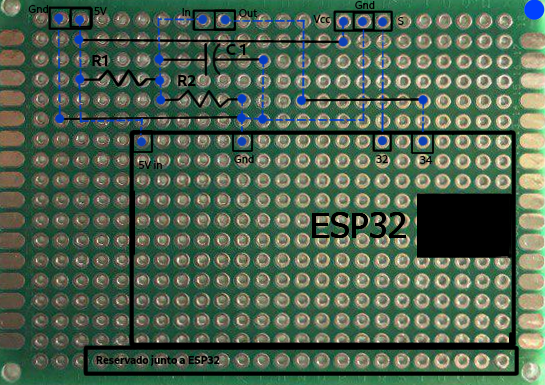
\includegraphics[width=0.8\textwidth]{img/dibujo_placa_vista_superior_arriba_y_abajo.png}
  \caption{Vista superior de la placa, en negro componentes y cableado
  de la parte anterior. En azul, de la parte posterior.}\label{fig:placa-sup-arriba-abajo}
\end{figure}

Hacemos uso del condensador $C1 = 10\mu F$ para absorber los
posibles picos de tensión, reducir el ruido en las lecturas y
garantizar calidad en las mismas.

Las resistencias $R1=R2=2k\Omega$ cumplen la función de un divisor de
tensión y de resistencia de carga para garantizar el voltaje operativo
del sensor de corriente y otorgar el rango de voltaje de salida esperado.

Para complementar esta visualización añadimos la parte posterior (trasera) de la
vista trasera de la placa (volteo vertical), Figura~\ref{fig:placa-tras-inf},
y la parte posterior de la vista superior, Figura~\ref{fig:placa-sup-inf}.

\begin{figure}
  \centering
  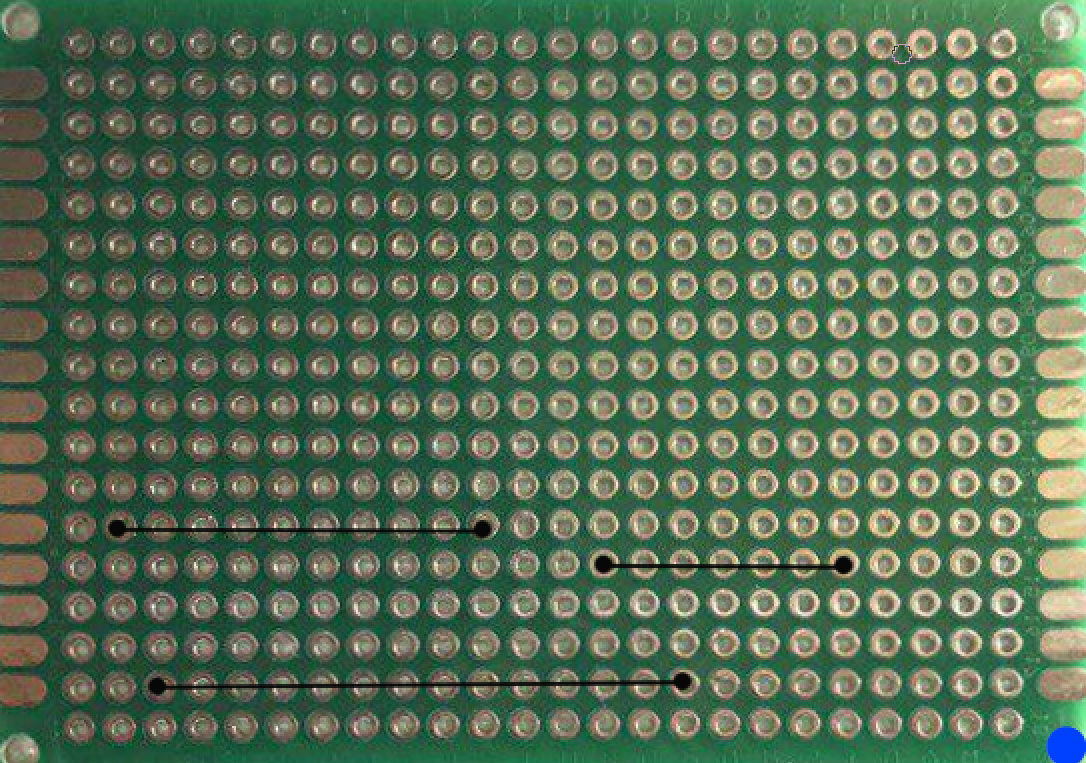
\includegraphics[width=0.8\textwidth]{img/dibujo_placa_vista_inferior_parte_trasera.png}
  \caption{Vista trasera de la placa, parte posterior.}\label{fig:placa-tras-inf}
\end{figure}

\begin{figure}
  \centering
  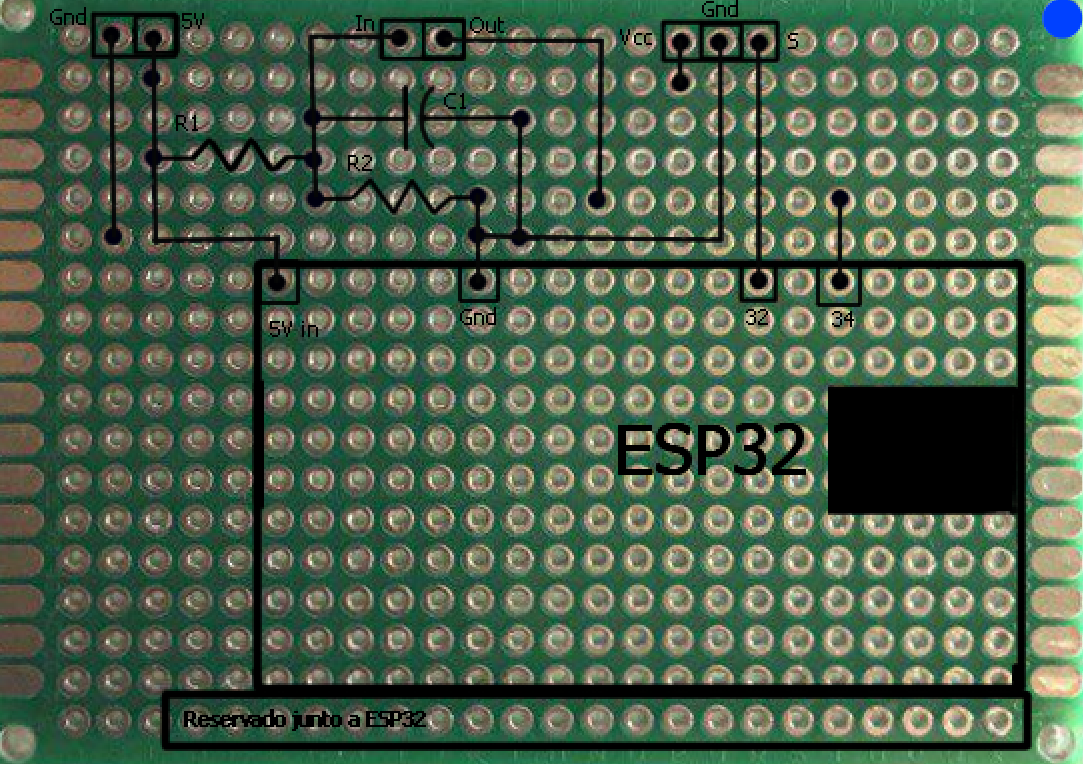
\includegraphics[width=0.8\textwidth]{img/dibujo_placa_vista_superior_parte_trasera.png}
  \caption{Vista trasera de la placa, parte posterior.}\label{fig:placa-sup-inf}
\end{figure}

Los adaptadores de los pines sobre los que se colocarán las otras
componentes queda dispuestos de acuerdo a la
Figura~\ref{fig:visual-adaptadores}. Hacemos uso de estos adaptadores
a fin de simplificar las tareas de mantenimiento y sustitución de
componentes en caso de avería.

\begin{figure}
  \centering
  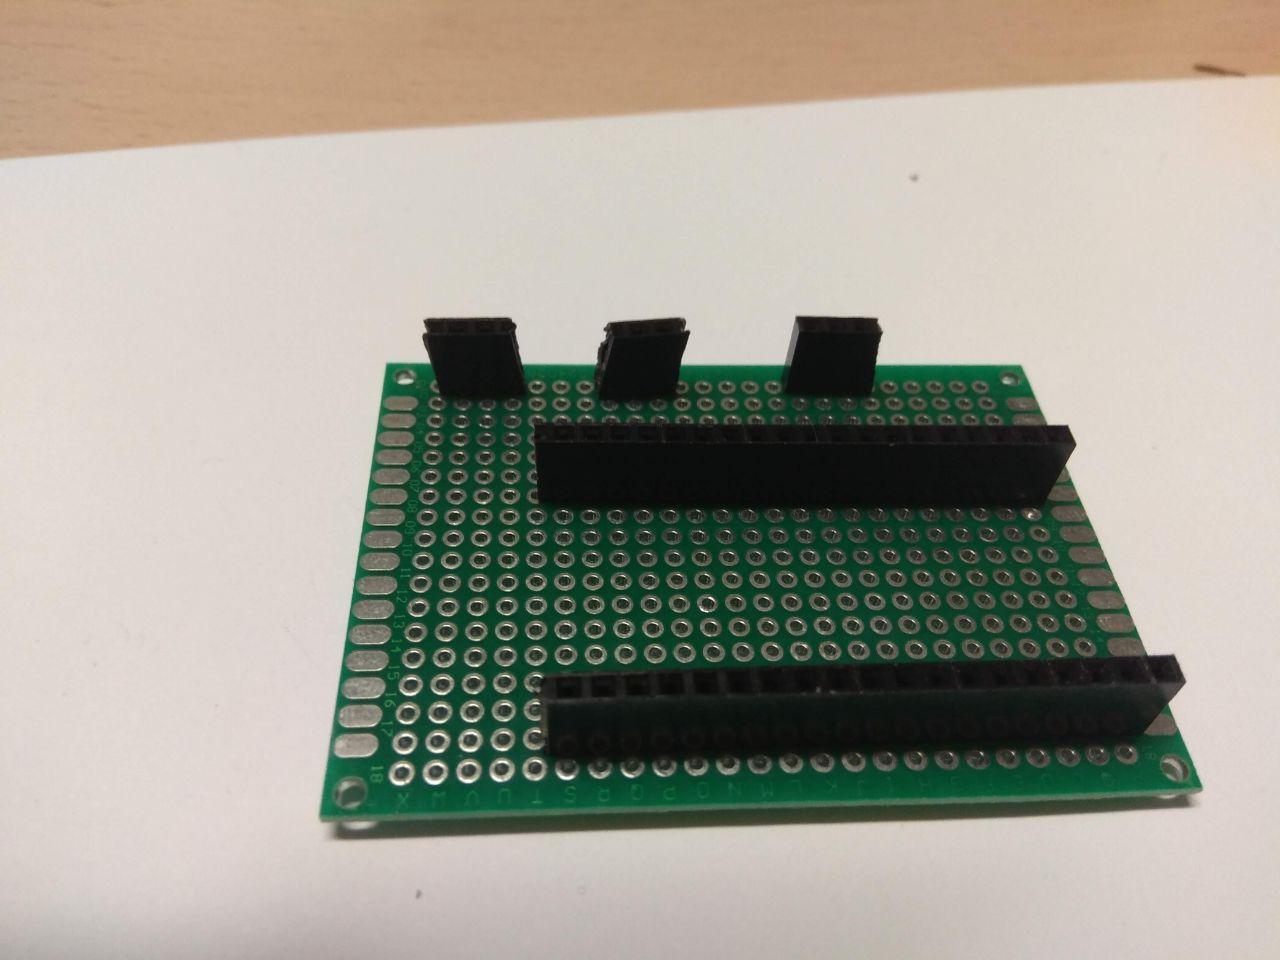
\includegraphics[width=0.8\textwidth]{img/placa_con_adaptadores_pines.jpg}
  \caption{Adaptadores de las componentes.}\label{fig:visual-adaptadores}
\end{figure}

El circuito resultante es el que podemos observar en las
figuras~\ref{fig:soldado_superior} y~\ref{fig:soldado_inferior}.

\begin{figure}
  \centering
  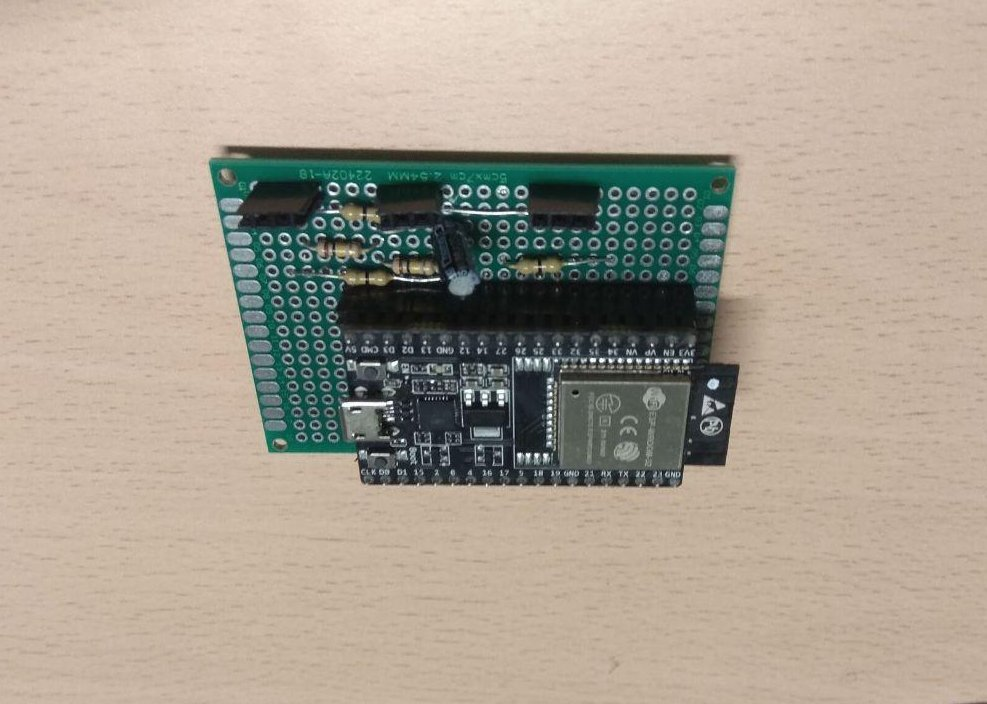
\includegraphics[width=0.8\textwidth]{img/soldadura_superior.jpg}
  \caption{Soldadura parte superior placa.}\label{fig:soldado_superior}
\end{figure}

\begin{figure}
  \centering
  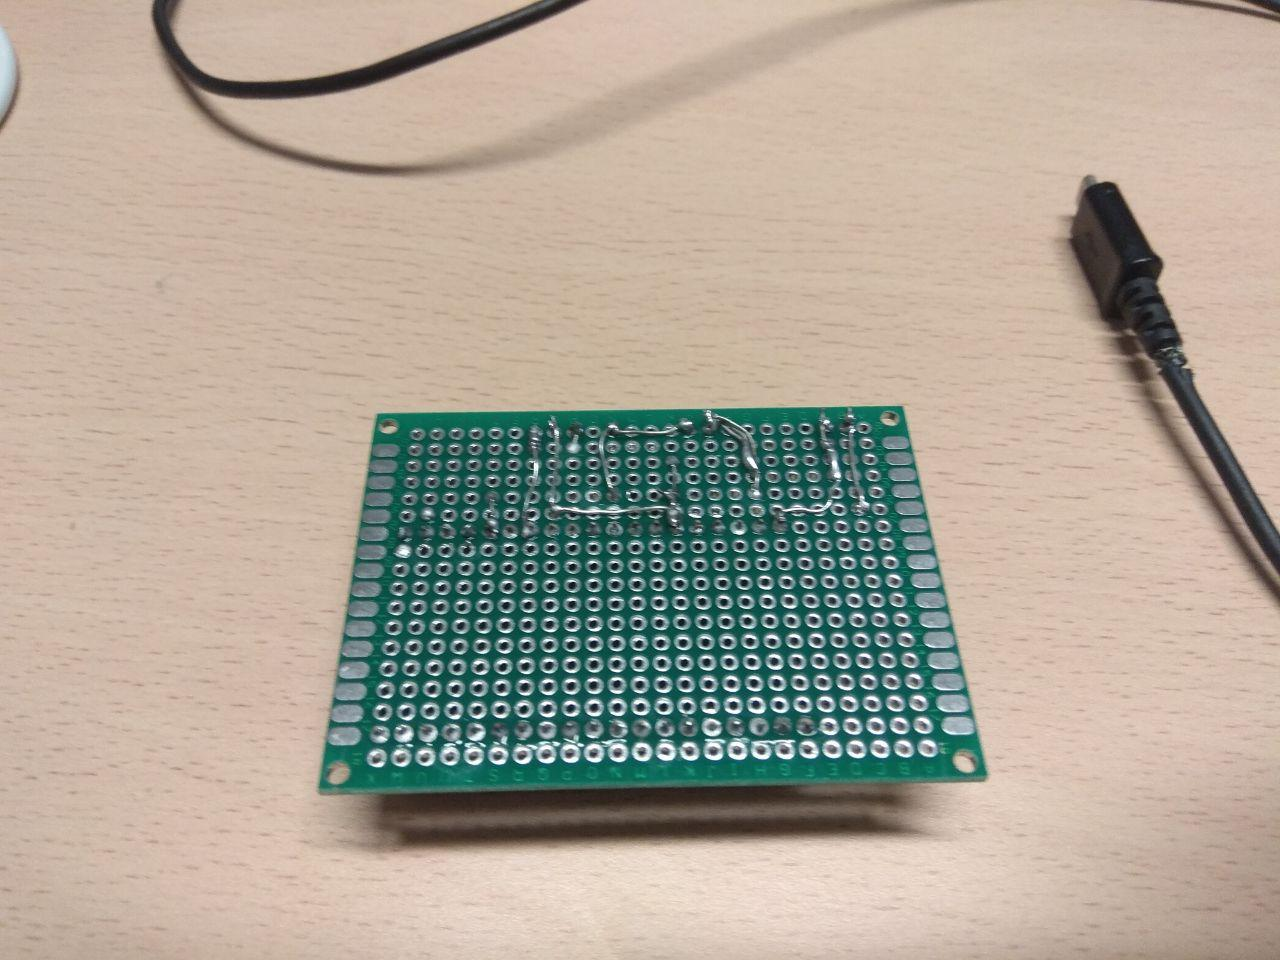
\includegraphics[width=0.8\textwidth]{img/soldadura_inferior.jpg}
  \caption{Soldadura parte inferior placa.}\label{fig:soldado_inferior}
\end{figure}

Tanto la alimentación como la medición de la corriente se produce a
partir de un cable que hemos seccionado y empalmado a las componentes
de nuestro circuito.

Para abstraer el diseño del enchufe y simplificar el uso del mismo al
usuario lo hemos acoplado en una caja de conexión. De este modo el
usuario final puede limitarse a, simplemente, conectar el dispositivo
a medir a nuestro enchufe inteligente y este a una fuente de
alimentación. Una conexión macho y una hembra.

\subsubsection{Programa del microcontrolador}

Toda la lógica del enchufe, tanto lecturas como comunicaciones, son
gestionadas por el programa del microcontrolador. Y resulta conveniente
comprender qué elementos hacen posible esta mecánica.

Por un lado se encuentra la configuración de la comunicación. Es
necesario conectarse a la red sobre la que se trabajará para poder
comunicarse con el broker, así que se requiere conocer SSID y
contraseña de la red en la que se trabajará. Del mismo modo la
información del broker, temas MQTT de suscripción o publicación y
credenciales tendrán que ser conocidos. Dada la licencia permisiva de
este proyecto y la flexibilidad de programación del módulo ESP32 no
habrá problema en entregar el sistema al usuario final en el estado de
uso inmediato o de permitir que este lo adapte a sus necesidades.

El enchufe publica el cálculo del consumo en un tema asociado a su
identificador en el broker y se suscribe a los canales de control para
gestionar su funcionamiento (actualmente manejo del relé, pero puede
extenderse a configuración de otros parámetros).

A fin de procesar la información del consumo cada enchufe está
identificado unívocamente por un identificador que puede ser adaptado
\textit{ad-hoc} (se podrían utilizar otros idendificadores como el del propio
microcontrolador, pero se deja a opción del usuario para permitir
flexibilidad en la nomenclatura).

En el apartado de las lecturas es destacable cómo se han realizado los
cálculos.

En términos de electromagnetismo se define la potencia W (la variable
que utilizamos para medir el consumo) como:

\[W = V\cdot A\]

Siendo V el voltaje del circuito, 230 voltios en España, y A la
intensidad de la corriente que mide el sensor.

Con las mediciones del sensor de corriente calculamos la
media cuadrática. La corriente alterna fluctúa en torno a valores
positivos y negativos siguiendo un comportamiento sinusoidal. La
manera de calcular la intensidad que realmente está pasando es
obteniendo el valor eficaz. Este valor eficaz para la intensidad se
corresponde con el valor cuadrático
medio\cite{alcaldesanmiguelElectrotecniaInstalacionesElectricas2014}.

Para reducir hipotéticos picos de ruido se realiza un muestreo un
intervalo de tiempo fijo y se calcula el consumo durante ese período
de tiempo \textit{W} tomando como valor de la corriente \textit{A} la
media de las medidas en el muestreo.

\newpage

\subsection{Servidor central}\label{subsec:servidor-central}

En el centro de nuestra arquitectura de estrella se encuentra el
servidor central. Una Raspberry Pi 3 Modelo B que actúa como broker
entre los publicadores y suscriptores de MQTT, como mencionábamos
en~\ref{subsubsec:broker_mosquitto}, haciendo uso de Mosquitto para
gestionar las publicaciones y suscripciones a los temas.

Es necesario que el broker esté activo y sea persistente a reinicios y
caídas. Por esto hay que configurarlo para que Mosquitto se lance en
cada inicio del servidor.

Este servidor supone el nodo central de nuestra topología de red, es
por tanto el más determinante para el correcto funcionamiento del
sistema. Si quisiéramos mejorar la disponibilidad del sistema para
poder seguir utilizándolo aunque este servidor esté caído puede ser
una mejora utilizar un segundo servidor similar a este al cual el
resto de nodos tomaran por broker en caso de que el primero estuviera
inaccesible.

\subsubsection{Configuración de red}

Para favorecer la localización del servidor central en la red es
conveniente asignarle bien una IP estática (configurar alguna interfaz
o modificar la configuración del cliente dhcp en Raspberry Pi) o bien
utilizar algún DNS y que se actualice la dirección de la misma.

En este caso hemos asignado una IP estática al servidor dentro de
nuestra red y hemos solicitado un nombre de dominio que actualiza la
IP pública del router de acceso al servidor, configurando además un
reenvío de puertos para que un cliente pueda conectarse desde el exterior.

\subsubsection{Gestión de la base de datos}

En el servidor central se encuentra situada una base de datos donde se
recogen las lecturas de los enchufes. De este modo se puede gestionar
la difusión de esta información a los clientes sin comprometer la
consistencia de los datos.

La estructura de esta base de datos consiste en una tabla que
incorpora para cada medición una fila con los datos del enchufe en el
que se ha leído, el consumo y la hora registrada según el servidor.

\newpage

\subsection{Aplicación de escritorio}

El último eslabón de nuestro sistema es el cliente de escritorio. Una
aplicación que permite al usuario final interactuar con el resto del
sistema.

Este cliente es en realidad una interfaz que otorga control sobre las
funcionalidades del sistema: Por un lado, acceder a la información
sobre el consumo eléctrico y visualizarla y, por otro lado, manipular
los enchufes inteligentes para controlar su estado.

En la topología de nuestro diseño este tipo de nodo forma parte de los
nodos periféricos que se conectan al servidor central. Pero a
diferencia de los otros nodos periféricos, los enchufes inteligentes,
estos permiten una mayor flexibilidad y libertad de configuración. Por
esto se le permite al cliente modificar desde la aplicación los
parámetros de conexión.

Una vez conectado al servidor la aplicación puede obtener la
información del mismo. Consultar su base de datos para obtener el
consumo realizado y poder visualizarlo de manera sencilla o consultar
los registros en mayor profundidad.

Al obtener esta información también estamos consultando qué enchufes
se encuentran conectados y qué identificadores tienen. Lo cual nos
permitirá controlar el estado de los enchufes (modificando el estado
de su relé) publicando en el broker en los temas de control a los que
los enchufes estarán suscritos.

\newpage

\section{Pruebas y test}

\textit{Aquí se adjuntarán algunas imágenes y resultados de los tests
  que se realicen sobre distintas partes del sistema}

\newpage

\section{Conclusión}

Ya sabíamos que el Internet de las Cosas traía consigo innumerables
posibilidades para extender la concepción habitual de los objetos que
nos rodean en nuestro día a día.

Con este proyecto se pretende hacer ver que el Internet de las Cosas
no es un concepto distante y que no existe una barrera económica o
tecnológica que solo permita a grandes empresas trabajar con él. El
Internet de las Cosas es accesible para cualquiera tanto para su uso
como para su desarrollo. Apto para cualquiera sin requerir grandes
gastos económicos y con unas opciones de diseño y desarrollo que
existen y que cada vez están mejor documentadas.


\newpage

\bibliographystyle{unsrt}
\bibliography{biblio} 

\end{document}
